\subsection{Lösungsansatz: Prediktive Kodierung}
Prediktoren sind typische Ansätze für verlustfreie Kompressionsverfahren. Die Frage ist, wie Informationen gelöscht werden. In erster Linie werden zwei Subsampling verfahren getestet, ein einfaches Subsampling und das Adaptive Subsampling. Das Adaptive Subsampling ist gut in unwichtige Informationen zu löschen, ist aber schwieriger zu kodieren. Das 

\subsubsection{Variante: einfaches Subsampling}
Für die erste Variante wird das Subsampling des DCT-Lösungsansatzes verwendet. Es reduziert die Punktmenge auf die Anzahl des Ist-Zustands. Die Feldlinien werden mit einer PCA in ein lokales Koordinatensystem transformiert. Im lokalen System können die Koordinaten mit 16 Bit Genauigkeit dargestellt werden. 16 Bit im Koordinatensystem der Sonne reichen nicht aus und führen zu einem grösseren Fehler als der Ist-Zustand.\\
In dieser Variante wird der Einfluss von vier Prediktoren getestet ($x$ sind die Bekannten Punkte und $y$ die Vorhersage):
\begin{itemize}
\item Konstanter Prediktor: Nimmt an, dass der nächste Wert im Kanal gleich dem  letzten Wert ist ($x = y$).
\item Linearer Prediktor: Nimmt an, dass die Steigung die Steigung zum nächsten Wert konstant bleibt ($x_1+(-x_2+x_1) = y$).
\item Linearer Prediktor mit Moving Average: Nimmt die durchschnittliche Steigung der letzten Werte.
\item Adaptiver Linearer Prediktor mit Moving Average: Berücksichtigt den Fehler der letzten Vorhersage.
\end{itemize}

\begin{figure}[!htbp]
	\center
	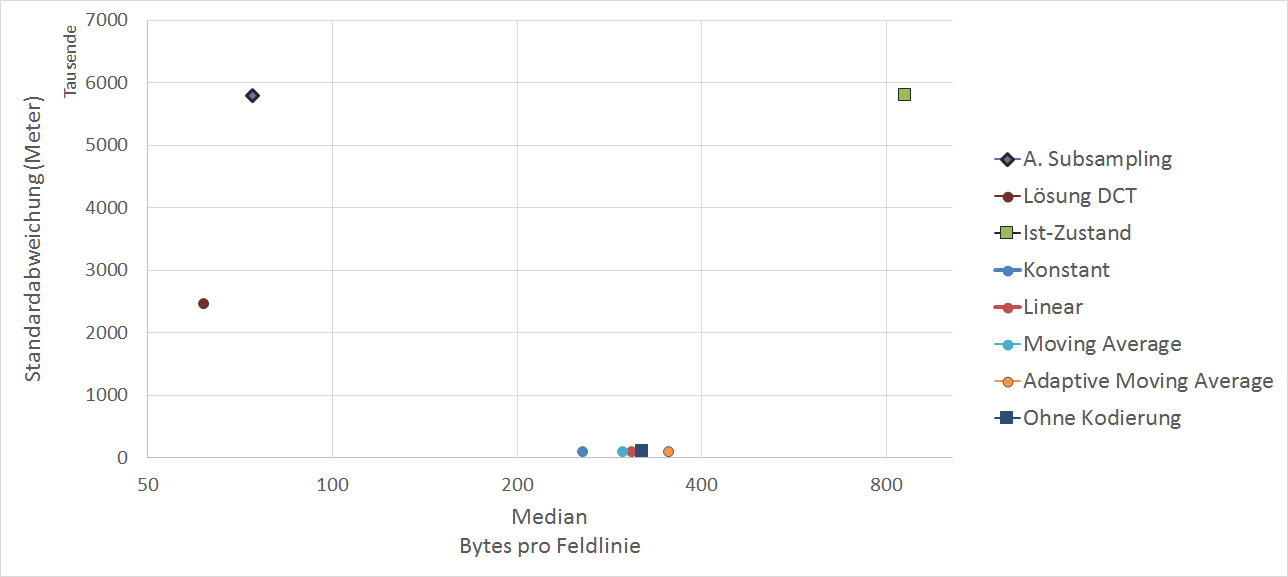
\includegraphics[width=1\textwidth,keepaspectratio]{./pictures/resultate/loesung2/variante0/resultate.png}
	\caption{Kompressionsraten der vier Prediktoren im Vergleich zum Ist-Zustand.}
	\label{resultate:loesung2:simple:resultate}
\end{figure}
Im Diagramm der Abbildung \ref{resultate:loesung2:simple:resultate} sind die Kompressionsraten der jeweiligen Prediktoren dargestellt. Ein Diagramm mit der PSNR-HVS-M wurde nicht erstellt. Sie ist für alle Prediktoren gleich und liegt bei $140.7$ dB. Unerwartet ist, dass der Konstante Prediktor mit $255$ Bytes pro Feldlinie die beste Kompression erreichte, obwohl die Daten nicht zuverlässig vorhersagen kann. Im Vergleich mit dem Moving Average Prediktor sind die Fehler der Vorhersagen 
bis zu $5$ Mal grösser, verbrauchen aber $40$ Bytes weniger um eine Feldlinie abzuspeichern. Der Fehler bleibt jedoch Konstant. Eine Möglichkeit ist, dass die Rar Kodierung sich wiederholende Muster findet.\\
Eine mögliche Optimierung ist die Adaptive Byte Kodierung der DCT-Variante, beschrieben im Abschnitt \ref{konzept:loesung1:kodierung}. Das Diagramm der Abbildung \ref{resultate:loesung2:simple:resultate_byte} zeigt die Resultate mit der Byte Kodierung. Der Konstante Prediktor verbraucht mit der Adaptiven Kodierung mehr Speicherplatz. Die Kompressionsrate der anderen Prediktoren wird durch die Adaptive Kodierung deutlich verbessert. Der Lineare Prediktor erreicht mit $214$ Bytes pro Feldlinie die beste Kompression. Das bedeutet, dass die Fehler des Konstanten Prediktors grösser sind, als die der anderen Prediktoren. Es bestätigt die Vermutung, dass die anderen Prediktoren die Daten besser vorhersagen können. Die Kompressionsrate des Konstanten Prediktors ist auf die Rar Kodierung zurückzuführen, welche in den Prediktor-Fehler Muster erkennen und effizient kodieren kann.\\ 
\begin{figure}[!htbp]
	\center
	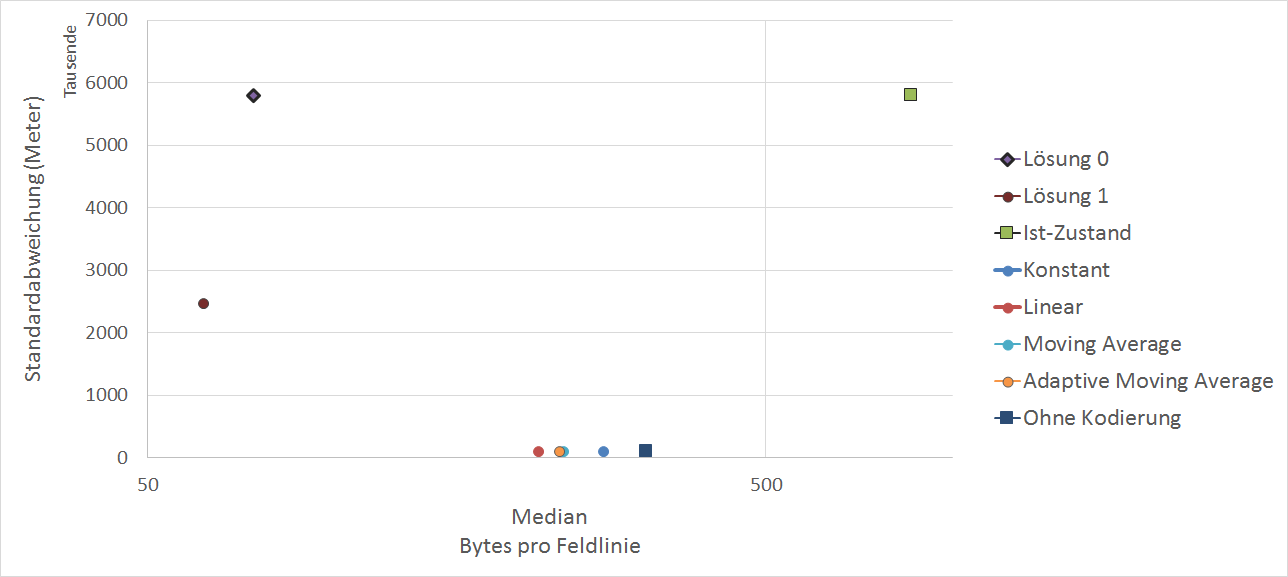
\includegraphics[width=1\textwidth,keepaspectratio]{./pictures/resultate/loesung2/variante0/resultate_byte.png}
	\caption{Kompressionsraten der Prediktoren mit Adaptiver Byte Kodierung.}
	\label{resultate:loesung2:simple:resultate_byte}
\end{figure}
Der Linare Prediktor kann eine Feldinie mit etwa $214$ Bytes darstellen, was eine Kompressionsrate von $4$ ergibt.

\subsubsection{Variante: Adaptives Subsampling}
Um mit diesem Ansatz in die selbe Grössenordnung zu gelangen wie die Lösungsansätze Adaptives Subsampling und DCT müssen mehr Informationen gelöscht werden. Es werden andere Parameter verwendet und im Schnitt $50\%$ mehr Punkte übertragen als im Lösungsansatz des Adaptiven Subsampling.\\
\begin{figure}[!htbp]
	\center
	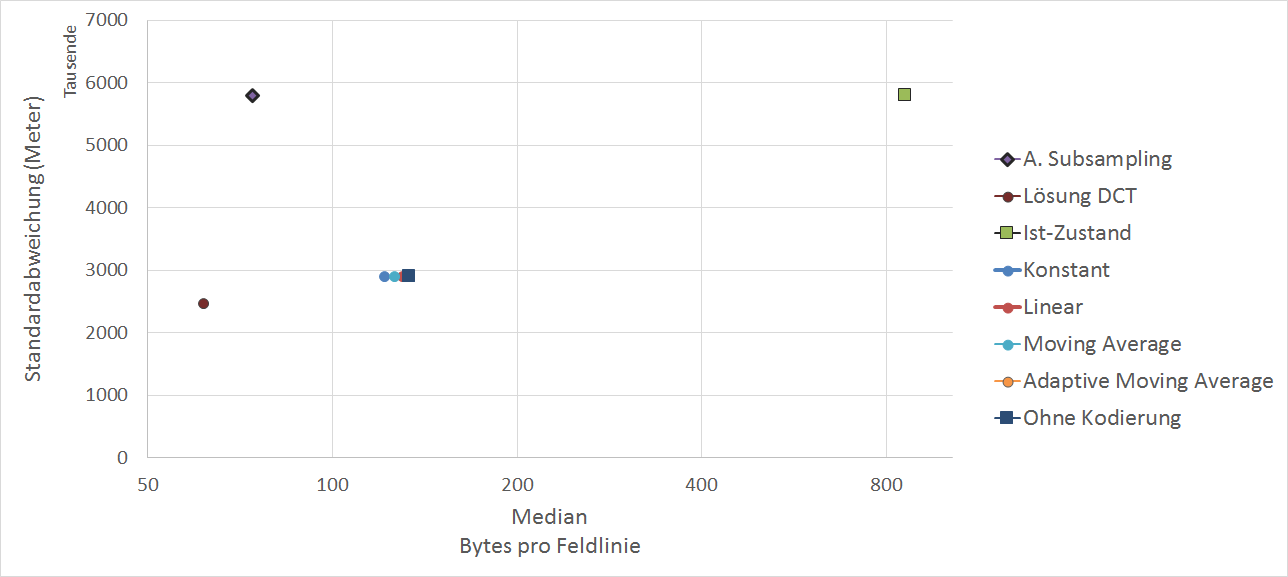
\includegraphics[width=1\textwidth,keepaspectratio]{./pictures/resultate/loesung2/variante1/resultate_euler.png}
	\caption{Kompressionsraten der Prediktiven Kodierungen mit dem adaptiven Subsampling.}
	\label{resultate:loesung2:adaptive:euler}
\end{figure}
Das Diagramm der Abbildung \ref{resultate:loesung2:adaptive:euler} zeigt die Kompressionsraten. Die Resultate liegen dicht beieinander und der Abstand zwischen Kodierung und der Kompression, welche ohne Kodierung erreicht wird wurde drastisch vermindert. Die Kodierungen erreichen eine PSNR-HVS-M von $139,2$. Das Angle Subsampling verändert die Eigenschaften der Daten. Die Diagramme der Abbildung \ref{resultate:loesung2:adaptive:channel} visualisiert die Veränderung. Monotone Steigungen sind nach dem Subsampling nicht mehr vorhanden. Die einfachen Prediktoren können die Daten nicht zuverlässig vorhersagen. 
\begin{figure}[!htbp]
	\center
	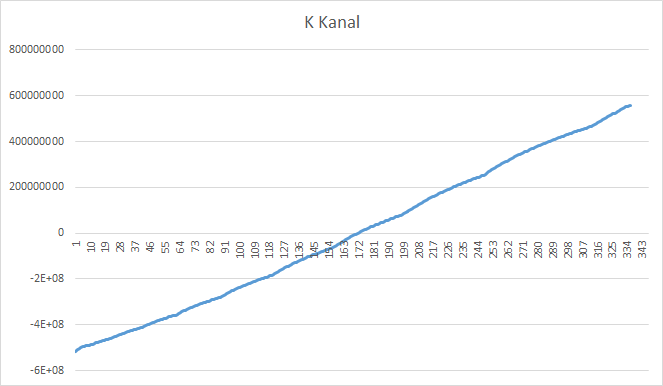
\includegraphics[width=0.49\textwidth,height=5cm,keepaspectratio]{./pictures/resultate/loesung2/variante1/channel_sub.png}
	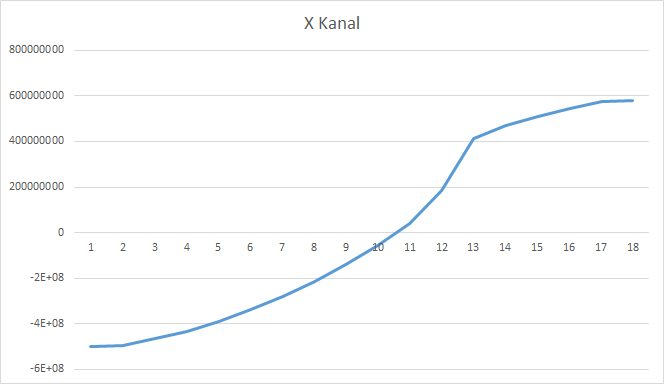
\includegraphics[width=0.49\textwidth,height=5cm,keepaspectratio]{./pictures/resultate/loesung2/variante1/channel_angle.png}
	\caption{Änderung der Eigenschaften der Daten durch das Angle Subsampling. Links der Kanal einer Feldlinie vor, rechts der Kanal nach dem Angle Subsampling.}
	\label{resultate:loesung2:adaptive:channel}
\end{figure}

\subsubsection{Rekursive Lineare Kodierung} \label{resultate:loesung2:wavelet}
Die Rekursive Lineare Kodierung ist in der Lage nicht-stetigen Kanälen eine sinnvolle Vorhersage zu berechnen. Das Verfahren ist im Abschnitt \ref{konzept:prediktiv} genauer erleutert. Die Punkte werden ins sphärische Koordinatensystem überführt. In diesem Koordinatensystem sind 16 Bit Genauigkeit pro Koordinatenachse ausreichend und die PCA muss nicht berechnet werden. Im Schnitt können dadurch $30$ Bytes pro Feldlinie eingespart werden. 
Zusätzlich werden die Vorhersagefehler quantisiert. Bei den einfachen Prediktoren wurde keine Quantisierung des Fehlers vorgenommen. Jede Quantisierung führte zu einem markanten Anstieg der Abweichung.\\
\begin{figure}[!htbp]
	\center
	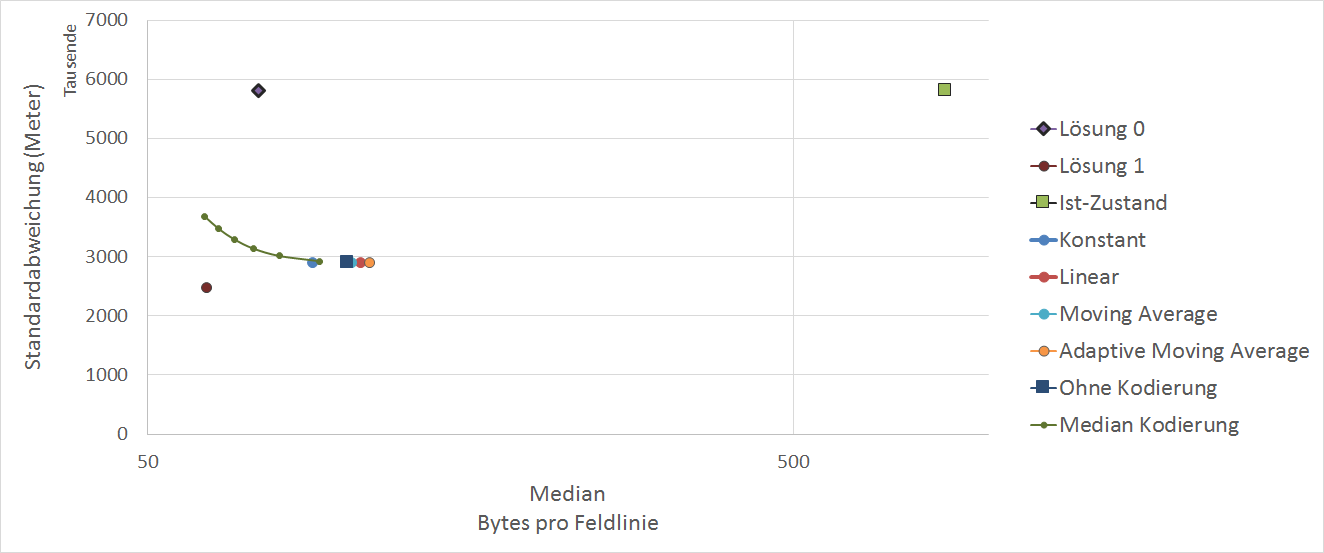
\includegraphics[width=1\textwidth,keepaspectratio]{./pictures/resultate/loesung2/variante2/resultate.png}
		\label{resultate:loesung2:adaptive:median}
		\caption{Kompressionsraten der Rekursive Lineare Kodierung mit dem adaptiven Subsampling.}
\end{figure}
\begin{figure}[!htbp]
	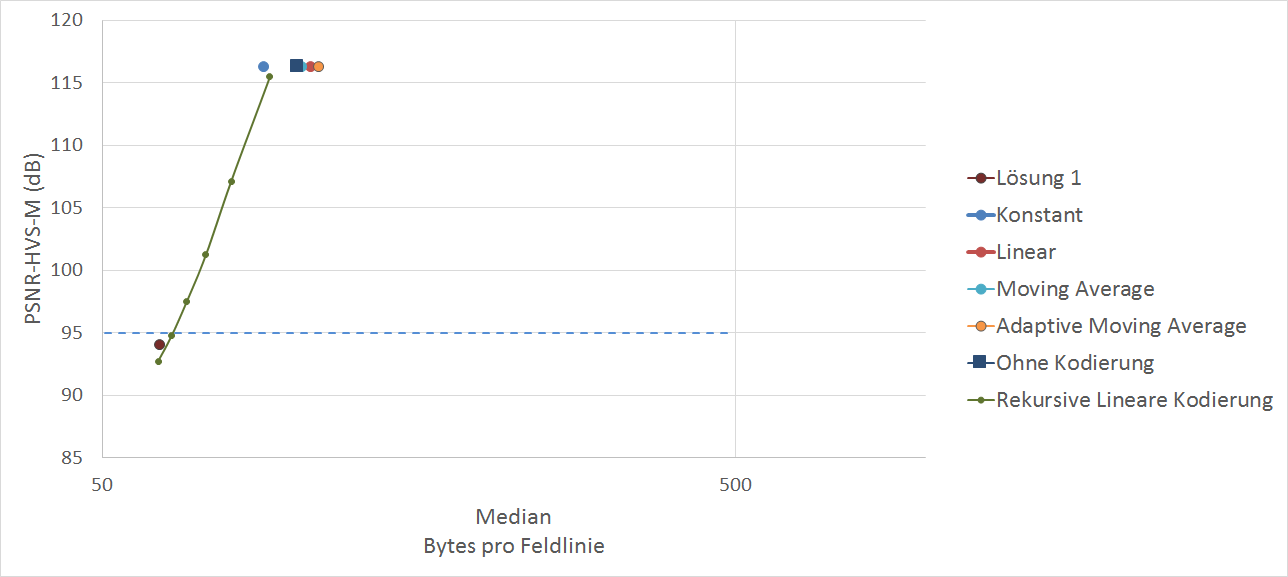
\includegraphics[width=1\textwidth,keepaspectratio]{./pictures/resultate/loesung2/variante2/resultate_psnr.png}
	\label{resultate:loesung2:adaptive:median_psnr}
	\caption{Kompressionsraten der Rekursive Lineare Kodierung mit dem adaptiven Subsampling.}
\end{figure}
Das Diagramm der Abbildung \ref{resultate:loesung2:adaptive:median} zeigt die Standardabweichung der Rekursiven Linearen Kodierung zu unterschiedlichen Quantisierungen. Das Diagramm der Abbildung \ref{resultate:loesung2:adaptive:median_psnr} zeigt die PSNR-HVS-M Werte der Variante. Die Resultate der einfachen Prediktoren wurden ebenfalls ohne PCA im sphärischen Koordinatensystem gemessen. Die Rekursive Lineare Kodierung kann eine bessere Kompressionsrate erreichen als die Lösung des Adaptiven Subsamplings. Bei Datenmenge von $64$ Bytes pro Feldlinie erreicht diese Variante eine tiefere Standardabweichung als das Adaptive Subsampling zu einem PSNR-HVS-M Wert von $94.7$. Dieser Ansatz besitzt weniger ausgeprägte Artefakte als die DCT Lösung, weist aber eine höhere Standardabweichung auf. Die Variante erreicht eine Kompressionsrate von $13.4$ und fällt somit zwischen den Lösungsansätzen DCT und Adaptives Subsampling.

Die Artefakte der Dekompression äussern sich meist als Verschiebungen einzelner Punkte. Im Extremfall können Ringing ähnlichen Artefakte entstehen, welche in der Abbildung \ref{resultate:loesung2:adaptive:median:artefakte} dargestellt sind. Die Artefakte sind weniger stark ausgeprägt als die des DCT Lösungsansatzes. Der Grund für die Artefaktbildung liegt in der Rekursion: Wenn der Vorhersagefehler des ersten Wertes (siehe Diagramm der Abbildung \ref{konzept:loesung2:algorithm:step1}) quantisiert wird, beeinflusst der Quantisierungsfehler den gesamten Kanal. Die Werte, welches als letztes Kodiert werden, erfahren die grösste Verschiebung bei der Dekompression. Diese Variante verwendet einen konstanten Faktor für die Quantisierung. Die Lösung ist eine angepasste Quantisierung, welche die ersten Vorhersagefehler mit höherer Genauigkeit abspeichert. 

\begin{figure}[!htbp]
	\center
	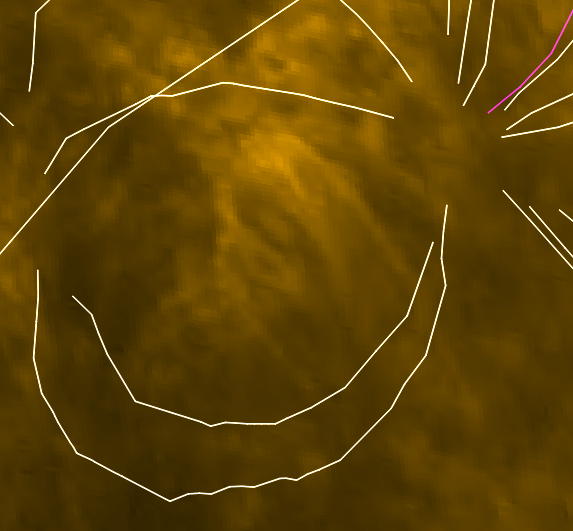
\includegraphics[width=0.8\textwidth,height=5cm,keepaspectratio]{./pictures/resultate/loesung2/variante2/artefakte1.png}
	\caption{Artefakte der Rekursiven Linearen Kodierung.}
	\label{resultate:loesung2:adaptive:median:artefakte}
\end{figure}

\subsubsection{Rekursive Lineare Kodierung mit angepasster Quantisierung}
Um die Artefakte der Dekompression zu dämpfen werden die Vorhersagefehler der Rekursionsstufe angepasst quantisiert. Die ersten Rekursionsstufen werden mit höherer Genauigkeit abgelegt.

Figure
Durch die angepasste Quantisierung konnte weiter Genauigkeit gewonnen werden und liegt nun fast gleichauf mit der DCT Lösung. Die Artefakte 

Artefakte wurden ebenfalls verbessert. Eine leichte Glättung ist aber dennoch willkommen, da sonst alles ein wenig wirr ist.
Durch die veränderte Quantisierung konnte weiter an Genauigkeit gewonnen werden. Das Diagramm der Abbildung



Das Caching von $1000$ Simulationen und die Übertragungszeit fallen zwischen die anderen Lösungsansätzen mit $73$ Megabyte an Arbeitsspeicher beziehungsweise $59$ Sekunden Übertragungszeit. Zum Vergleich: Die DCT Lösung verbraucht unter den selben Bedingungen $70$ und das Adaptive Subsampling $85$ Megabyte an Arbeitsspeicher. Bei einer Internetverbindung von $10$ Megabit ist bei diesem Lösungsansatz mit einer Übertragungsrate von $16$ Simulationen in der Sekunde zu rechnen. Die Laufzeit der Dekompression liegt mit $30.6$ Millisekunden ebenfalls zwischen den Lösungsansätzen Adaptives Subsampling und DCT. Mit dieser Laufzeit kann ein Thread durchschnittlich $32$ Simulationen pro Sekunde dekomprimieren.

Dieser Lösungsansatz ist ein Kompromiss zwischen Kompressionsrate und Qualität. Die Daten enthalten Kompressionsartefakte. Sie sind aber schwach ausgeprägt sodass auf eine Glättung gegebenenfalls verzichtet werden kann.